\documentclass[tikz,border=5pt]{standalone}
\usetikzlibrary{calc}
\begin{document}
% Scale s = 0.008484 cm/px (longest side 943 px -> 8 cm); centre cx=546.5, cy=454.5
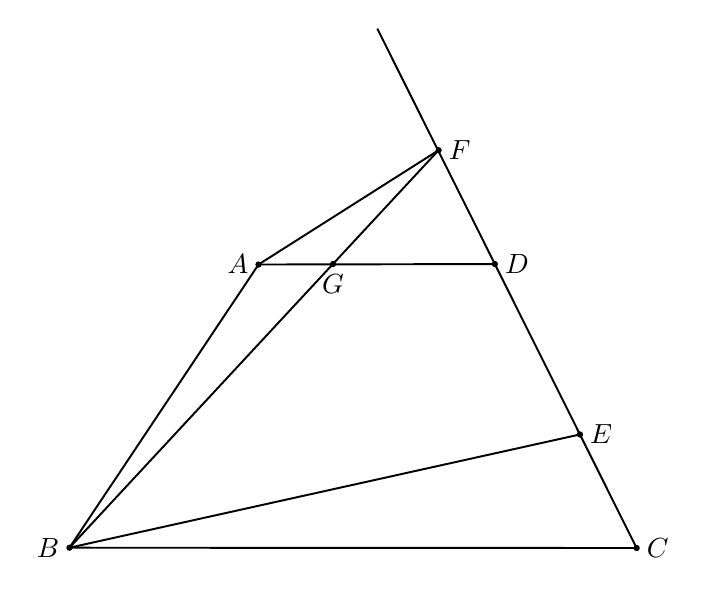
\begin{tikzpicture}[line width=0.7pt, line join=round, every node/.style={font=\fontsize{10}{12}\selectfont}]

% Named coordinates (pixel -> cm)
\coordinate (A) at (-1.2047,0.3886);
\coordinate (B) at (-3.6057,-3.2078);
\coordinate (C) at (3.5972,-3.2116);
\coordinate (D) at (1.7968,0.3945);
\coordinate (E) at (2.8771,-1.7698);
\coordinate (F) at (1.0826,1.8404);
\coordinate (G) at (-0.2588,0.3945);
\coordinate (X) at (0.3037,3.3843); % far end of line C-F, past F

% Segments (geometry unchanged)
\draw (B) -- (C);            % B-C
\draw (A) -- (D);            % A-D (through G)
\draw (C) -- (X);            % C-E-D-F extended past F
\draw (A) -- (F);            % A-F
\draw (B) -- (A);            % B-A
\draw (B) -- (E);            % B-E
\draw (B) -- (F);            % B-F (through G)

% Points
\foreach \p in {A,B,C,D,E,F,G} \fill (\p) circle (0.04);

% Labels: anchors adjusted to match original placement
\node[left]  at (A) {$A$};   % left of A
\node[left]  at (B) {$B$};   % left of B
\node[right] at (C) {$C$};   % right of C
\node[right] at (D) {$D$};   % right of D
\node[right] at (E) {$E$};   % unchanged
\node[right] at (F) {$F$};   % right of F
\node[below] at (G) {$G$};   % directly below G
\end{tikzpicture}
\end{document}